\documentclass{standalone}
\usepackage{tikz}
\usepackage{ctex,siunitx}
\usepackage{tkz-euclide}
\usepackage{amsmath}
\usetikzlibrary{patterns, calc}
\usetikzlibrary {decorations.pathmorphing, decorations.pathreplacing, decorations.shapes,}
\begin{document}
\small
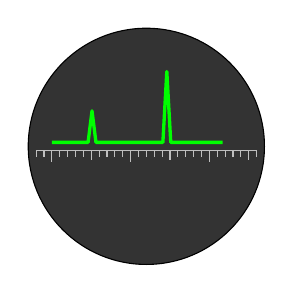
\begin{tikzpicture}[>=latex,scale=1.0]
  % \useasboundingbox(-1,1.2)rectangle(5,2.8);
  \draw[fill=black!80] (0,0) circle (1.5);
  \draw [lightgray,thin](-1.4,-0.05)--(1.4,-0.05);
  \foreach \x in {-1.2,-0.2}
  {
    \draw[lightgray,thin](\x,-0.05)--++(0,-0.15);
    \foreach \y in {1,2,3,4,6,7,8,9}
    {
      \draw[lightgray,thin](\x+\y*0.1,-0.05)--++(0,-0.08);
    }
    \draw[lightgray,thin](\x+0.5,-0.05)--++(0,-0.12);
  }
  \foreach \x in {-1.4,-1.3,0.9,1.0,1.1,1.2,1.4}
  {
    \draw[lightgray,thin](\x,-0.05)--++(0,-0.08);
  }
  \draw[lightgray,thin](1.3,-0.05)--++(0,-0.12);
  \draw[lightgray,thin](0.8,-0.05)--++(0,-0.15);
  \draw [very thick,green,line join=round] (-1.2,0.05)--++(0.46,0)--++(0.05,0.4)--++(0.05,-0.4)--++(0.85,0)--++(0.05,0.9)--++(0.05,-0.9)--++(0.66,0);
  \end{tikzpicture}
\end{document}